%%%
%%% FORMAL GAP IDENTIFICATION
%%%
\section{Deriving the Gap to Ordinary Transformation}

%\todo{Exchange "ordinary" with "unidirectional"}
We have already introduced that there is both a formal and practical gap between synchronizing transformations, as we have defined as a component of transformation networks, and ordinary transformations, which are unidirectional and non-synchronizing, as used by most transformation languages.
In the following, we first give an example for faulty behavior if we simply used ordinary transformations in a transformation network.
Afterwards, we give a formal definition of unidirectional preservation rules and ordinary transformations, then defined as \emph{bidirectional transformations}.
Finally, we discuss the relation between unidirectional consistency preservation rules and unidirectional consistency relations as introduced in \autoref{chap:compatibility:formal_notion}.
%discuss options to sequence ordinary transformations and finally come up with a precise description of the formal gap and a practical approach to close it.


%%
%% MOTIVATING FAULT EXAMPLE WITH ORDINARY TRANSFORMATIONS
%%
\subsection{Behavior of Ordinary Transformations in Networks}
We have already sketched the example of creating a class in UML and Java after adding a component to a \gls{PCM} model in \autoref{chap:introduction:challenges:correctness:synchronization}.
In that scenario, it was possible that for a created \gls{PCM} component first a UML class is generated, which is then transformed into a Java class.
Additionally, the transformation between \gls{PCM} and Java creates another Java class, as it does not consider that there may be another transformation that already created that class.
Such scenarios can lead to the duplication of elements as an already existing element is inserted again, or to an overwrite of an already existing element.
Overwriting a previously created element may also overwrite and thus remove information that was already added to that it, like the transformation across UML may have added information to the Java class which is overwritten by new class creation of the transformation from PCM to Java.

\begin{figure}
    \centering
    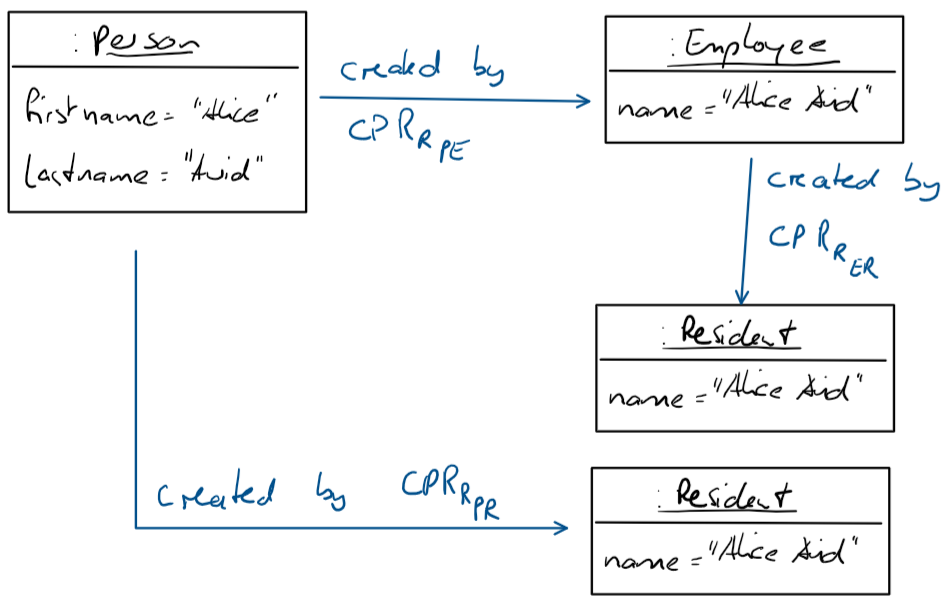
\includegraphics[width=0.8\textwidth]{figures/correctness/synchronization/duplicate_creation_example.png}    
    \caption[Duplicate creation of an element]{Duplicate creation of a resident by two sequences of consistency preservation rules.}
    \label{fig:synchronization:duplicate_creation_example}
\end{figure}

An analogous example can be given for the running example of persons, employees and residents depicted in \autoref{fig:networks:three_persons_example}.
We consider the consistency relations $\consistencyrelation{R}{PE}, \consistencyrelation{R}{ER}$ and $\consistencyrelation{R}{PR}$.
As discussed in \autoref{chap:compatibility}, these relations are compatible, thus for any given person, employee or resident, there is a consistent tuple of models containing it.
Thus, the relations do not prevent transformations from finding consistent models whenever a person, employee or resident is added.
If we now consider ordinary transformations with unidirectional consistency preservation rules, they react to the changes in one model and update another accordingly.
In case of adding a person, this may look as depicted in \autoref{fig:synchronization:duplicate_creation_example}.
For each of the given consistency relations, we assume unidirectional consistency preservation rules that preserve consistency according to them.
They especially create an employee for each added person, and a resident for each created employee and person, respectively.
Since the transformations assume the models to be consistent before applying the changes, they always add a corresponding element when one of the elements is added.
This leads to the situation that both $\consistencypreservationrule{\consistencyrelation{CR}{ER}}$ as well as $\consistencypreservationrule{\consistencyrelation{CR}{PR}}$ create a resident upon creation of a person.
In consequence, there exist two residents with the same name, which does not fulfill the consistency relations.

It is our goal to find out how such a situation can be avoided by proper definition of consistency preservation rules in existing transformation languages.
A simple solution in this example would have been to look for the existence of elements to create first.
This can either be done by using a trace model, which most existing transformation language use to store corresponding elements, or by searching for an appropriate element in the other model.
Using a trace model, however, has some drawbacks and pitfalls, which we will investigate later.

% \begin{copiedFrom}{DocSym}

% % \section{Binary Transformation Interoperability}

% % Multi-model consistency preservation can be a achieved by combining binary transformations to graphs, %of transformations, 
% % with the transformations being executed transitively.
% % Since all binary transformations are developed independently of each other, it is necessary that they interoperate properly in a \emph{non-intrusive} way, thus without the necessity for the developer to understand and modify them, which we refer to as \emph{black-box combination}.

% Even under the assumption that, in contrast to our introductory motivation, all specifications are free of contradictions, it is easy to see that problems arise when combining binary transformations by transitively executing them.
% For example, consider the relations in \autoref{fig:prologue:binary_combination_example}.
% If a component is added to the \ac{ADL}, causing a \ac{UML} class creation due to \ref{fig:prologue:binary_combination_example:R1}, which in turn causes a Java class creation due to \ref{fig:prologue:binary_combination_example:R2}, the transformation for relation \ref{fig:prologue:binary_combination_example:R3} does not know that an appropriate class was already created, if the transformations are treated as black boxes.
% Consequently, the transformation will create the same class again, which may override the existing one, depending on the implementation and execution order.
% A simple solution for this example would be to have all transformations use a common trace model and check for existing elements before creating them in a transformation.
% Nevertheless, independently developed transformations will usually not assume that %this only applies if the transformation considers possibly preexisting transformation results, which it will not do in general if it does not assume other transformations to create corresponding elements.
% other transformations may already have created corresponding elements.
% Additionally, the trace model must allow the transformation engine to retrieve transitive traces.
% However, it is unclear if transitive resolution of traces can always be performed, as it can depend on whether the transitive trace belongs the considered consistency relation or another.
% %If, in another scenario, the transformation in the example was actually supposed to create an additional class, it would have to ignore the existing trace.

% As can be seen in the example, especially the correct handling of trace information in interdependent transformations has to be researched.
% This applies not only to element creations, but also other change types, such as attribute or reference changes, especially if they are multi-valued.
% In our thesis, we will therefore apply transitively executed binary transformations in different case studies to identify these and potential further problems.
% We then want to come up with a catalog of such problems %preventing the black-box combination of transformations 
% together with solution patterns for them.
% For example, to avoid duplicate element creations, a simple pattern could be to always check for already existing traces for that consistency relation in the transformations.
% In consequence, the integration of those patterns into a transformation language or the application of them as a transformation developer is supposed to achieve black-box combinability of the transformations.

% \end{copiedFrom} % DocSym

%%%%%%% MOVED TO CORRECTNESS CHAPTER
%%
%% USING FINE-GRAINED RELATIONS
%%
%%\subsection{Consistency Preservation of Fine-grained Relations}
%%\label{chap:synchronization:gap:finegrained}

% \mnote{Consistency preservation defined for model-level consistency relations}
% In our definition of consistency preservation rules in \autoref{def:consistencypreservationrule}, we used the coarse-grained notion of \modellevelconsistencyrelations, which describe consistency between two models in terms of a single relations.
% In consequence, such a \modellevelconsistencypreservationrule ensures consistency to a single consistency relation.

% \mnote{Fine-grained consistency relations allow to define relation between unidirectional preservation rules}
% In \autoref{chap:compatibility:formal_notion}, we discussed that consistency relations can be considered in a fine-grained way that is able to reflect different notion of consistency in both directions between two models, such as a employee requiring a resident to exist but not vice versa.
% We thus refined the notion of consistency relations in \autoref{def:consistencyrelation} to be defined unidirectionally and at the level of model elements rather than complete models.
% %This fine-grained notion of consistency does also fit well to how specifications in transformation languages consider consistency, as they define rules that relate only some classes by relations or routines to preserve their consistency.
% Since we also consider unidirectional consistency preservation rules as defined in transformation languages, we base further considerations regarding consistency preservation rules on such fine-grained and unidirectional consistency relations.
% We later discuss how unidirectional consistency relations and unidirectional consistency preservation rules are related.
% Nevertheless, we did also discuss in that chapter that each fine-grained relation can also be translated into a \modellevelconsistencyrelation, thus all insights we already had for those model-level relations still apply to the considerations regarding fine-grained ones.

% \mnote{Transformation languages use fine-grained relations and preservation rules}
% This fine-grained notion of consistency does also fit well to how specifications in transformation languages consider consistency.
% They allow to define rules that relate only some classes by relations, conforming to fine-grained consistency relations, from which then fine-grained consistency preservation rules are derived, or they directly allow to define routines to preserve consistency between specific classes.
% These rules are often called \emph{transformation rules} and composed to a transformation that consists of multiple such rules, each encoding a consistency relations and a preservation rule for it.
% %We will, however, stick to the coarse-grained notion of consistency preservation rules, because, first, it is difficult to describe how such fine-grained consistency preservation rules can be composed, and second, the coarse-grained notion is sufficient for our considerations anyway.

% \mnote{Stick to coarse-grained notion of preservation rules}
% It may easily happen that the execution of one transformation rule leads to the violation of the consistency relation of another one, which introduced dependencies between the individual transformation rules.
% Thus, a combination of such transformation rules to a transformation has to ensure correctness, i.e., that the consecutive execution of the rules leads to a consistent state of the models.
% Languages such as \gls{QVTR} and \gls{QVTO} therefore specify that transformation rules may not be conflicting (cf. \cite[7.10.2.]{qvt}).
% It is also a dedicated topic of research to ensure that the rules of a single transformation conform to each other, e.g.\ \cite{cuadrado2017tse,cabot2010VerificationInvariants-JSS}, thus we assume that a transformation has that property.
% To avoid the necessity of specifying this conformance property for transformation rules, we stick to the existing notion of coarse-grained consistency preservation rules, as it is sufficient for our considerations.

% \mnote{New transformation notion based on fine-grained consistency relations}
% In consequence, from now we consider a synchronizing transformation as a set of fine-grained consistency relations according to \autoref{def:consistencyrelation} and a consistency preservation rule that preserves consistency according to the set of relations $\consistencyrelationset{CR}$ rather than a single \modellevelconsistencyrelation $\consistencyrelation{CR}{}$.
% A consistency preservation rule $\consistencypreservationrule{\consistencyrelationset{CR}}$ and also a transformation with that preservation rule are thus still considered correct if it is applied to a consistent pair of models and changes to them and applying the resulting changes to the models again delivers a pair of models that is consistent to all consistency relations, i.e.:
% \begin{align*}
%     &
%     \forall \model{m}{1} \in \metamodelinstanceset{M}{1}, \model{m}{2} \in \metamodelinstanceset{M}{2}, \change{\metamodel{M}{1}} \in \changeuniverse{\metamodel{M}{1}}, \change{\metamodel{M}{2}} \in \changeuniverse{\metamodel{M}{2}} : \tupled{\model{m}{1},\model{m}{2}} \consistenttomath \consistencyrelationset{CR} \\
%     & \formulaskip
%     \land \exists \change{\metamodel{M}{1}}' \in \changeuniverse{\metamodel{M}{1}}, \change{\metamodel{M}{2}}' \in \changeuniverse{\metamodel{M}{2}} : \tupled{\change{\metamodel{M}{1}}', \change{\metamodel{M}{2}}'} = \consistencypreservationrule{\consistencyrelationset{CR}}(\model{m}{1}, \model{m}{2}, \change{\metamodel{M}{1}}, \change{\metamodel{M}{2}}) \\
%     & \formulaskip\formulaskip
%     \Rightarrow \tupled{\change{\metamodel{M}{1}}'(\model{m}{1}),\change{\metamodel{M}{2}}'(\model{m}{2})} \consistenttomath \consistencyrelationset{CR}
% \end{align*}
% Note that being consistent to all fine-grained consistency relations is equivalent to being consistent to the single \modellevelconsistencyrelation induced by the fine-grained relations.

% In our definition of consistency preservation rules in \autoref{def:consistencypreservationrule}, we used the coarse-grained notion of \modellevelconsistencyrelations and, accordingly, defined \modellevelconsistencypreservationrules that consider models as whole.
% We refined the notion of consistency relations in \autoref{def:consistencyrelation} to be defined at the level of model elements rather than complete models.
% This fine-grained notion of consistency fits well to how specifications in transformation languages consider consistency, as they define rules that relate only some classes by relations or routines to preserve their consistency.
% In the following, we thus also stick to this fine-grained notion of consistency.
% We will, however, stick to the coarse-grained notion of consistency preservation rules given in \autoref{def:consistencypreservationrule}

% \subsection{Feingranulare CPR}
% Jede CPR stellt Konsistenz bzgl. einer unidirektionalen CR wieder her.
% Ein CPR darf keine Änderung machen, die eine andere CR verletzt.
% Schwierig, da CPR voneinander abhängen können (was wiederum dagegen spricht, dass eine CPR nicht eine andere CR verletzen darf), wie also Reihenfolge festlegen?
% Ist keine Option, insbesondere Annahme, dass sich CPR nicht gegenseitig beeinflussen nicht nachvollziehbar (obwohl in der Praxis dasselbe Probleme existiert, da CPR sowieso in feingranulare Regeln zerlegt werden, die natürlich widersprüchlich sein könnten).

%\todo{Relate to the circumstance that we want to consider unidirectional preservation rules, so unidirectional rules might be interesting. We will later find, that this is not the case}


%%
%% UNIDIRECTIONAL CONSISTENCY PRESERVATION RULES
%%
\subsection{Unidirectional Consistency Preservation Rules}

\mnote{Formal definition of unidirectional consistency preservation rules}
Before we can discuss options how unidirectional consistency preservation rules can be used to emulate the behavior of synchronizing consistency preservation rules, we first need to define them to be able to formally compare the two of them.
In contrast to a synchronizing consistency preservation rule as defined in \autoref{def:consistencypreservationrule}, a unidirectional consistency preservation rule does only receive changes made to one of the two models and returns changes to the other models instead of receiving and returning changes to both.

\begin{definition}[Unidirectional Consistency Preservation Rule]
    \label{def:unidirectionalconsistencypreservationrule}
    Let $\metamodel{M}{1}, \metamodel{M}{2}$ be two metamodels and $\consistencyrelationset{CR}$ a set of consistency relations between elements of those metamodels.
    A \emph{unidirectional consistency preservation rule} $\consistencypreservationrule{\consistencyrelationset{CR}}$ for the relation set $\consistencyrelationset{CR}$ is a (usually partial) function:
    \begin{align*}
        \consistencypreservationrule{\consistencyrelationset{CR}} : (\metamodelinstanceset{M}{1}, \metamodelinstanceset{M}{2}, \changeuniverse{\metamodel{M}{1}}) \rightarrow \changeuniverse{\metamodel{M}{2}} \cup \setted{\bot}
    \end{align*}
\end{definition}

\mnote{Preservation rules as defined in or derived from transformation languages}
This is how the consistency preservation rules defined in or derived from existing transformation languages operate.
They take two models and changes to one of them and generate changes for the other.
Most of them even directly apply the changes instead of returning a dedicated change artifact.
If the rule is not able to handle the given changes, it may return $\bot$.

\mnote{Correctness of unidirectional rules analogous to common notions}
In addition, they usually assume the input models to be consistent and then ensure that applying the input and the output changes to the models, the resulting models are consistent again.
This conforms to the common notion of \emph{correctness} for consistency preservation rules, like for the state-based (rather than our delta-based) notion of consistency preservation rules defined in \cite{stevens2010sosym}.
This is even compliant to the correctness notion that we defined for synchronizing consistency preservation rules in \autoref{def:consistencypreservationrulecorrectness}.
Thus, we define correctness of such a unidirectional consistency preservation rule as follows.

\begin{definition}[Unidirectional Consistency Preservation Rule Correctness]
    \label{def:unidirectionalconsistencypreservationrulecorrectness}
    Let $\consistencypreservationrule{\consistencyrelationset{CR}}$ be a unidirectional consistency preservation rule.
    We call $\consistencypreservationrule{\consistencyrelationset{CR}}$ \emph{correct} if the resulting models when applying the generated changes are consistent to $\consistencyrelationset{CR}$ again:
    \begin{align*}
        &
        \forall 
        \model{m}{1} \in \metamodelinstanceset{M}{1}, 
        \model{m}{2} \in \metamodelinstanceset{M}{2},
        \change{\metamodel{M}{1}} \in \changeuniverse{\metamodel{M}{1}} : \\
        & \formulaskip
        \bigl( \tupled{\model{m}{1}, \model{m}{2}} \consistenttomath \consistencyrelationset{CR} \\
        & \formulaskip
        \land \exists 
        \change{\metamodel{M}{2}} \in \changeuniverse{\metamodel{M}{2}} :
        \change{\metamodel{M}{2}} = \consistencypreservationrule{\consistencyrelation{CR}{}}(\model{m}{1}, \model{m}{2}, \change{\metamodel{M}{1}}) \bigr) \\
        & \formulaskip\formulaskip
        \Rightarrow
        \tupled{\change{\metamodel{M}{1}}(\model{m}{1}), \change{\metamodel{M}{2}}(\model{m}{2})} \consistenttomath \consistencyrelationset{CR}
    \end{align*}
\end{definition}

\mnote{Synchronizing consistency preservation rules can be partial}
In \autoref{def:unidirectionalconsistencypreservationrule}, we explicitly allow consistency preservation rules to be partial.
This was only an optional requirement for synchronizing consistency preservation rules defined in \autoref{def:consistencypreservationrule}, because there may be changes to both models which cannot be processed reasonably as one the changes may need to reverted to achieve consistency.
Ignoring that practical requirement, it is theoretically possible to always return changes that, if applied to the input models, produce consistent models.
Those returned changed may perform arbitrarily unreasonable modifications, but still restore consistency.

\mnote{Unidirectinoal consistency preservation rule must be partial}
In general, unidirectional consistency preservation rules need to be partial.
This is due to the reason that there can be models for which no other models can be generated such that they are consistent with respect to a set of consistency relations.
Consider the consistency relations $\consistencyrelation{CR}{} = \setted{\tupled{a, z}, \tupled{b, z}}$ and its transposed $\consistencyrelation{CR}{}^T = \setted{\tupled{z, a}, \tupled{z, b}}$.
If a change generated the model $\model{m}{} = \setted{a, b}$, then no consistent model can be generated.
A consistent model would have to contain $z$, because the consistency relation $\consistencyrelation{CR}{}$ requires for $a$ and $b$ an element $z$ to exist in the other model.
The consistency relation $\consistencyrelation{CR}{}^T$, however, requires that for a $z$ only either $a$ or $b$ exists in the other model, as otherwise no witness structure with unique corresponding elements can be found (see \autoref{def:consistency} for consistency).
In consequence, a unidirectional consistency preservation rule may not produce a result for such an input and thus be partial, as the result would never fulfill the correctness definition.

In fact, the definition does not specify for which inputs a unidirectional consistency preservation rule is allowed to be undefined.
One could restrict this behavior to cases in which there is no $\change{\metamodel{M}{2}} \in \changeuniverse{\metamodel{M}{2}}$ for given models $\model{m}{1}$ and $\model{m}{2}$ as well as change $\change{\metamodel{M}{1}} \in \changeuniverse{\metamodel{M}{1}}$, such that $\tupled{\change{\metamodel{M}{1}}(\model{m}{1}), \change{\metamodel{M}{2}}(\model{m}{2})} \consistenttomath \consistencyrelationset{CR}$ for a set of consistency relation $\consistencyrelationset{CR}$.
We, however, leave it up to the developer to decide for which inputs a consistency preservation rule is undefined, as there might be cases in which a change that restores consistency can be restored, but does semantically not make this.
This was also the reason for allowing a synchronizing consistency preservation rule to be partial, which is why we have already discussed the scenario in \autoref{chap:correctness:formalization:incremental_inductive}.
% \subsection{Partial Definition of Consistency Preservation Rules}
% \todo{Move this to definition of unidirectional preservation rules?}
% 1. Schon eine synchronisierende Transformation muss nicht für jede Eingabe definiert sein. Es könnte natürlich sein, dass sich gleichzeitige Änderungen nicht sinnvoll in Einklang bringen lassen. Theoretisch ist es aber möglich eine total definierte Funktion anzugeben, da immer ein beliebigen (im dümmsten Fall immer dasselbe / leere Modell) zurückgeliefert werden kann.


%%
%% NONALIGNMENT OF UNIDIRECTIONAL CONSISTENCY RELATIONS AND UNIDIRECTIONAL CONSISTENCY PRESERVATION RULES
%%
\subsection{Unidirectional Relations and Preservation} % Alignment}
\label{chap:synchronization:gap:alignment}

\mnote{Unidirectional consistency preservation rules for each unidirectional consistency relation}
Defining unidirectional consistency preservation rules based on a unidirectional notion of consistency relations imposes the idea of having one unidirectional consistency preservation rule associated with one unidirectional consistency relation, or at least a set of unidirectional relations between the same two metamodels.
In consequence, we would have two sets of unidirectional consistency relations between two metamodels and a consistency preservation rule for each of them.

\begin{figure}
    \centering
    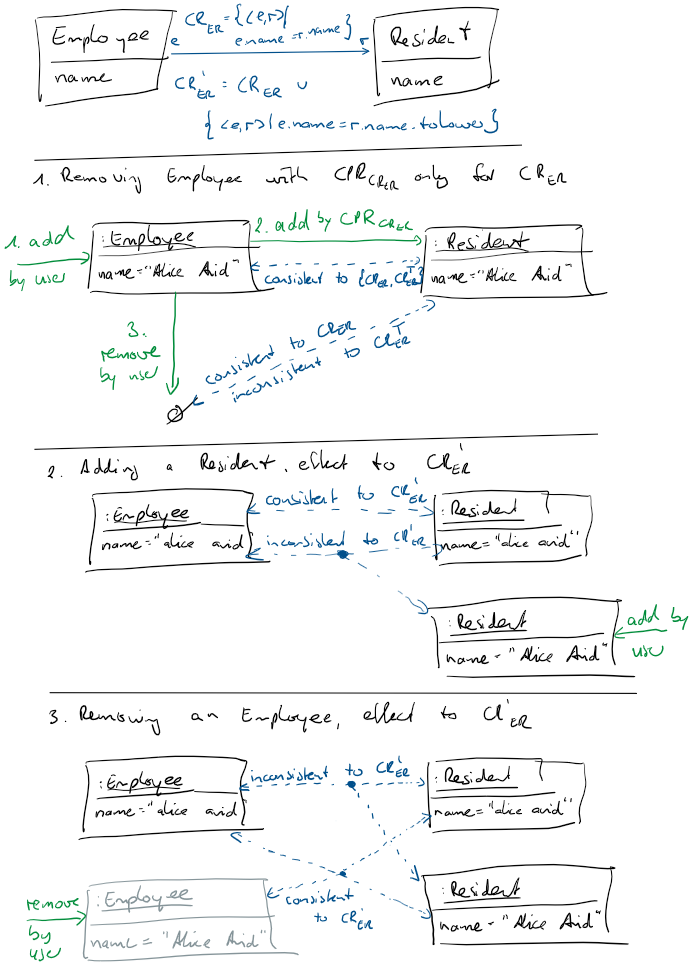
\includegraphics[width=0.85\textwidth]{figures/correctness/synchronization/unidirectional_nonalignment.png}
    \caption[Nonalignment of unidirectional relations and preservation]{Nonalignment of unidirectional relations and preservation rules. %: scenario for unidirectional consistency preservation rule requiring knowledge about consistency relation in opposite direction (1)
    }
    \todo{Split into two figures}
    \label{fig:synchronization:unidirectional_nonalignment}
\end{figure}

\mnote{Unidirectional consistency preservation rules cannot only consider one direction of consistency relations}
It is, however, easy to see that a unidirectional consistency preservation rule cannot only consider one direction of consistency relations, but needs to consider both.
Consider the example in \autoref{fig:synchronization:unidirectional_nonalignment}, which contains an extract of the consistency relations of the running example.
We assume the consistency relations $\consistencyrelation{CR}{ER}$ and $\consistencyrelation{CR}{ER}^T$ describing that for each employee a single corresponding resident must exist and vice versa.
As discussed before, only considering $\consistencyrelation{CR}{ER}$ would realize the notion of not requiring an employee for every resident.
If we define a unidirectional consistency preservation rule $\consistencypreservationrule{\consistencyrelation{CR}{ER}}$ only for the consistency relation $\consistencyrelation{CR}{ER}$ with the goal to always preserve consistency according to that relation after changes to the employee model, the example scenario 1 in \autoref{fig:synchronization:unidirectional_nonalignment} show that this is not the case.
While for the scenario of adding an employee the rule properly propagates the change by adding a resident and thus restores consistency, removing an employee leads to a violation of consistency.
Removing an employee does not require the consistency preservation rule to perform any changes in the resident model, because $\consistencyrelation{CR}{ER}$ only requires a unique resident to exist for every employee, but does not forbid that there is a resident for which no employee exists.
This is defined by the inverse relation $\consistencyrelation{CR}{ER}^T$.
In consequence, after removing tan employee the consistency preservation rule does not perform any changes, as consistency to $\consistencyrelation{CR}{ER}$ is given, but the model are then inconsistent to $\consistencyrelation{CR}{ER}^T$.

\mnote{Changes to one model may affect consistency relations in both directions}
The given scenario exemplifies the general case that a consistency according to a consistency relation cannot only be violated by performing changes to the model containing the left condition elements of the relations, but also by changes to the model containing the right condition elements of the relation.
In general, consistency of models according to a consistency relation is affected by the presence of condition elements in the models.
Consistency is defined as the ability to find a witness structure, i.e., a unique mapping between condition elements of the consistency relation that occur in the models.
Thus, adding, changing or removing elements in model that constitute a condition element of the consistency relations can lead to inconsistencies.

\mnote{Distinction of addition, removal or change of condition elements for consistency relation affection}
We can see that any type of change can lead to the violation of a consistency relation in either direction:
\begin{properdescription}
    \item[Addition:] Whenever a condition element of the left side of a consistency relation is added to a model, a corresponding condition element need to exist in the other model. If it does not exist yet, the models are not consistent to that relation.
    When a condition element of the right side of a consistency relation is added to a model, this does, according to the definition of consistency, not require another condition element to exist in the other model. It can, however, lead to the situation that no witness structure with a unique mapping between the elements exists anymore.
    Consider the exemplary relation $\consistencyrelation{CR}{ER}'$ in \autoref{fig:synchronization:unidirectional_nonalignment} and the example scenario 2.
    Having an employee with name \enquote{alice avid} and a corresponding resident with the same name, the models are consistent to that relation.
    Adding a resident with name \enquote{Alice Avid} violates $\consistencyrelation{CR}{ER}'$, because the employee \enquote{alice avid} corresponds to both residents, so there is no mapping inducing a witness structure for consistency.
    In consequence, adding a right side condition element of the consistency relation to the models can also violate consistency to a consistency relation.
    \item[Removal:] Whenever a condition element of the right side of a consistency relation is removed from a model, the corresponding condition element in the other model still exists. Because this element does not necessarily have a corresponding one anymore, there may not be a valid witness structure and thus the models may not be consistent anymore.
    When a condition element of the left side of a consistency relation is removed from a model, the originally corresponding element is not connected to the removed element in the witness structure anymore. If another element is considered to this corresponding element, there is no unique mapping of elements anymore.
    Consider again the relation $\consistencyrelation{CR}{ER}'$ in \autoref{fig:synchronization:unidirectional_nonalignment} and the example scenario 3.
    Having two employees and residents with the names \enquote{alice avid} and \enquote{Alice Avid}, the models are consistent because each employee has a corresponding resident and vice versa.
    If we remove the employee \enquote{Alice Avid}, the models are consistent to $\consistencyrelation{CR}{ER}'$ anymore, because the remaining employee corresponds to both residents, so there is no unique mapping of condition elements.
    \item[Change:] We do not have a precise notion of when a condition element can be considered changed, as elements do not have identity. 
    Additionally, consistency in terms of being able to find a witness structure is only based on the existence or non-existence of condition elements, thus whether an element was changed or removed and created makes no different.
    We might say that a condition element can be considered changed when the change describes modifications of the model elements in the condition element that lead to a new condition element within the same condition.
    This does, conceptually, not different from the removal of one and the addition of another condition element.
    Thus, the same situations as discussed for addition and removal above can occur.
\end{properdescription}

\mnote{Unidirectional consistency preservation rules cannot be synchronizing}
%In addition to the insight that unidirectional consistency preservation rule must base on all consistency relations between two metamodels rather than only the ones in a specific direction, 
It is also easy to see that there is no trivial way of specifying a unidirectional synchronizing consistency preservation rule.
It may seem natural to define a consistency preservation rule that is able to process changes in both models and then return only changes in one of them to restore consistency to close the gap between synchronizing and ordinary transformations.
Consider the situation that we have two residents and employees named \enquote{Alice Avid} and \enquote{Bob Do}.
If one of them is removed in the residents model and the other in the employees model, then a proper synchronizing transformation should remove both corresponding elements such that the models are empty.
This requires changes to both models.
With a synchronizing unidirectional consistency preservation rule for each direction, neither of them can produce changes in one of the models that reasonably restore consistency.
Such a rule would necessarily revert one removal to restore consistency, which is not the intended behavior and would probably not be specified by a developer that way, such that the consistency preservation rule would be undefined for that input, although a synchronization transformation would be able to resolve those changes.
In fact, we would expect to have two unidirectional consistency preservation rules of which each removes one of the elements.
This does, however, violate our existing notion of correctness for a single consistency preservation rule.
In the subsequent sections, we will therefore discuss relaxed requirements to unidirectional consistency preservation rules to be able to act like a synchronizing transformations.

% A unidirectional consistency relations require preservation rules in both directions (add/delete)
% \begin{itemize}
%     \item A single unidirectional consistency relation may impose preservation rules in both directions: For each employee, a resident is required, but not every resident needs to be an employee. When then have only one unidirectional consistency relation describing that circumstance. We need, however, consistency preservation rules in both directions, because if, for example, a resident is removed, the employee needs to be removed as well, whereas a resident has to be added whenever an employee is added.
%     \item With ordinary unidirectional rules, we then have that after a change to model 1, the unidirectional rule has to change model 2 so that they are consistent to both unidirectional relations (and vice versa)
% \end{itemize}
% Konsequenz: Wir können nicht für die unidirektionalen Konsistenzrelationen jeweils die CPR in die Richtung angeben, sondern jede unidirektionale CPR muss immer die Konsistenzrelationen in beide Richtungen berücksichtigen.

% Define mapping between change types and directionality of involved consistency relation (delete in opposite direction than add or modification). Make example at witness structures.

% Beachten, dass auch beim Hinzufügen in m2 die Relation m1->m2 verletzt werden kann, da nun zu viele Elemente vorhanden sind -> keine Witness-Struktur.


% \paragraph{Synchronizing Transformation cannot be Unidirectional}
% Es ist einfach zu sehen, dass synchronisierende Transformationen nicht so einfach unidirektional definiert werden können.
% Wird m1 beliebig geändert und in m2 ein Element gelöscht, welches für Konsistenz zu m1 notwendig war, dann kann die unidirektionale CPR m2 nicht wieder so anpassen, dass es konsistent zu m1 ist, außer indem es das gelöschte Element wieder hinzufügt. Hier wäre es richtig das Element in m1 durch die gegenläufige CPR zu löschen. 
% Das bedeutet aber das Korrektheit hier nicht definiert werden kann als die Eigenschaft Konsistenz bzgl. aller CR durch eine unidirektionale CPR herzustellen.

% Das gilt allerdings nur, wenn man den Korrektheitsbegriff beibehält. Wir werden sehen, dass es andere Möglichkeiten gibt diesen Begriff einer unidirektionalen synchronisierenden Transformation zu definieren.


%%
%% COMPOSING TWO UNIDIRECTIONAL CPR TO BIDIRECTIONAL TRANSFORMATIONS
%%
\subsection{Bidirectional Transformations}

\mnote{Unidirectional consistency preservation rules usually appear as pairs}
A unidirectional consistency preservation rule does usually not appear on its own but in combination with another rule for the opposite direction.
We have already seen that even a single unidirectional consistency relation between two metamodels requires unidirectional consistency preservation rules for both directions to preserve consistency according to that relation after changes either instances of either of the metamodels.
In practice, many transformation languages, especially relational ones such as \gls{QVTR} or \gls{TGG} tools, allow the specification of \emph{bidirectional transformations}, which means that they define or derive unidirectional consistency preservation rules for both directions.

\mnote{Combine two unidirectional consistency preservation rules to a bidirectional transformation}
In general, it is reasonable to consider two unidirectional consistency preservation rules between two metamodels together, such that after changes in instances of any of the two metamodels, the other model can be updated to restore consistency.
A synchronizing transformation according to \autoref{def:synchronizingtransformation} is also able to process changes in any of the two models, thus such a notion fits to our goal of emulating synchronizing transformations.
According to common terminology, we define this as a bidirectional transformation.

\begin{definition}[Bidirectional Transformation]
    \label{def:bidirectionaltransformation}
    Let $\metamodel{M}{1}$ and $\metamodel{M}{2}$ be two metamodels and $\consistencyrelationset{CR}$ a set of consistency relations between them.
    Additionally, let $\consistencypreservationrule{\consistencyrelationset{CR},{\rightarrow}}$ and $\consistencypreservationrule{\consistencyrelationset{CR},{\leftarrow}}$ be unidirectional consistency preservation rules with:
    \begin{align*}
        &
        \consistencypreservationrule{\consistencyrelationset{CR}}^{\rightarrow} : (\metamodelinstanceset{M}{1}, \metamodelinstanceset{M}{2}, \changeuniverse{\metamodel{M}{1}}) \rightarrow \changeuniverse{\metamodel{M}{2}} \cup \setted{\bot} \\
        &
        \consistencypreservationrule{\consistencyrelationset{CR}}^{\leftarrow} : (\metamodelinstanceset{M}{2}, \metamodelinstanceset{M}{1}, \changeuniverse{\metamodel{M}{2}}) \rightarrow \changeuniverse{\metamodel{M}{1}} \cup \setted{\bot}
    \end{align*}
    A \emph{bidirectional transformation} is a triple $\transformation{t} = \tupled{\consistencyrelationset{CR},\consistencypreservationrule{\consistencyrelationset{CR}}^{\rightarrow}, \consistencypreservationrule{\consistencyrelationset{CR}}^{\leftarrow}}$.
\end{definition}

\mnote{Correctness of bidirectional transformations}
We call such a bidirectional transformation correct if both consistency preservation rules are correct, i.e., they both preserve consistency according to the underlying consistency relation set.

\begin{definition}[Bidirectional Transformation Correctness]
    \label{def:bidirectionaltransformationcorrectness}
    Let $\transformation{t} = \tupled{\consistencyrelationset{CR}, \consistencypreservationrule{\consistencyrelationset{CR}}^{\rightarrow}, \consistencypreservationrule{\consistencyrelationset{CR}}^{\leftarrow}}$ be a bidirectional transformation.
    We call $\transformation{t}$ correct if, and only if, $\consistencypreservationrule{\consistencyrelationset{CR}}^{\rightarrow}$ and $\consistencypreservationrule{\consistencyrelationset{CR}}^{\leftarrow}$ are both correct according to \autoref{def:unidirectionalconsistencypreservationrulecorrectness}.
\end{definition}

\mnote{Bidirectional transformations do not support changes of both models}
Such bidirectional transformations ensure that if any of two models is changed, a change for the other is generated such that both changed models are consistent again, if possible.
This does, however, not reflect the case that both models have been modified concurrently, as it is the case in transformation networks and thus supported by our initial definition of synchronizing transformations.
We therefore discuss in the following sections how we can combine the unidirectional consistency preservation rules of a bidirectional transformation and which requirements we have to make to them such that the bidirectional transformation behaves like a synchronizing one.

